\documentclass[conference]{IEEEtran}
\IEEEoverridecommandlockouts
\usepackage{cite}
\usepackage[utf8]{inputenc}
\usepackage[english]{babel}
\usepackage{bookmark}
\usepackage[square,sort,comma,numbers]{natbib}
\usepackage{listings}
\usepackage{url}
\usepackage{wrapfig}
\usepackage{caption}
\usepackage{color}
\usepackage{enumitem}
\usepackage{graphicx}
\usepackage{float}
\usepackage{url}
\def\UrlBreaks{\do\/\do-}
\usepackage{breakurl}
\graphicspath{{images/}}
\usepackage{hyperref}

\def\BibTeX{{\rm B\kern-.05em{\sc i\kern-.025em b}\kern-.08em
    T\kern-.1667em\lower.7ex\hbox{E}\kern-.125emX}}

\begin{document} 
    \title{
        Assignment 3\\[0.3cm]
        \large  Deep Convolutional Neural Networks\\
        ELE494-09
    }

    \author{
        \IEEEauthorblockN{Nasir Khalid}
        \IEEEauthorblockA{b00065082\\}
    }

    \maketitle

    \section{Importing CIFAR-10 Dataset}

    This was done using the keras.datasets object. They were imported as
    training and testing images. Along with training and testing labels.
    Shown below is an output from the code that displays their shape and randomly
    displays a single image from the dataset.

    \begin{figure}[H]
        \centering
        \captionsetup{justification=centering}
        \centering
            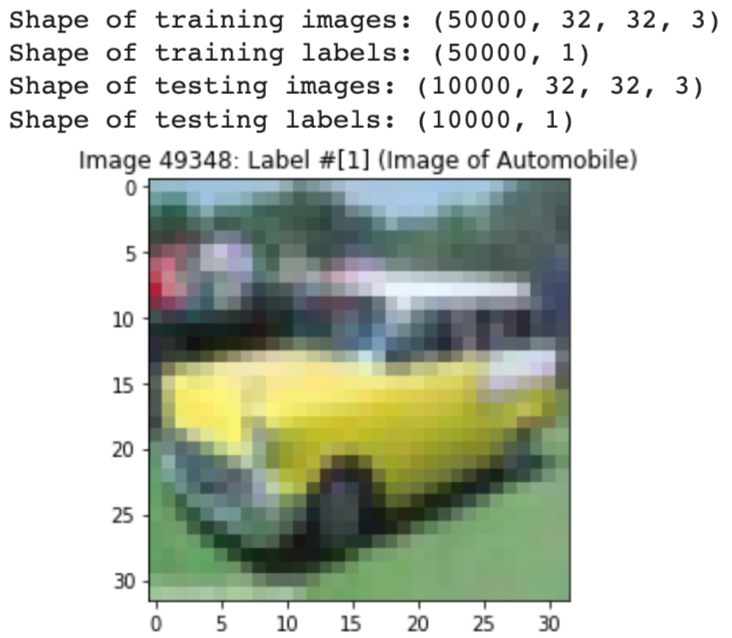
\includegraphics[width=0.3\textwidth]{1.png}
            \caption{Data set shapes and random image from dataset}
    \end{figure}


    \section{Design Your Own Architecture}

    For this step I created a custom architecture that consists of 4 convolution
    layers and 2 max pooling layers. The final few layers consist of 2 dense layers
    and the final softmax layer for the output. Batch size is 32. A summary is shown below
    
    \begin{figure}[H]
        \centering
        \captionsetup{justification=centering}
        \centering
            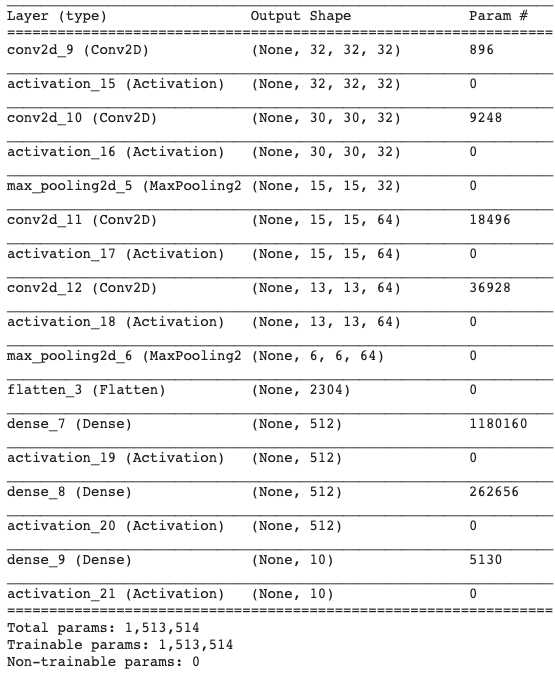
\includegraphics[width=0.28\textwidth]{2.png}
            \caption{Summary of initial architecture}
    \end{figure}

    There are a total of 1513514 parameters. When this network was trained it performed
    poorly with a final loss value of 14.4988 and a validation loss of 14.5740 and an
    accuracy of 10\% with a validation accuracy of 9.58\%. On the test data
    the accuracy was 10\%. Shown below are the accuracy and loss curves for this network.

    \begin{figure}[H]
        \centering
        \captionsetup{justification=centering}
        \centering
            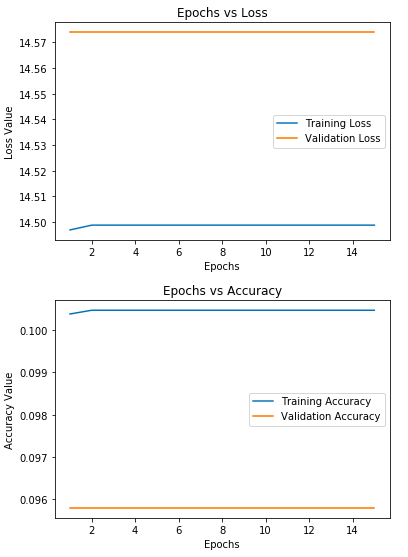
\includegraphics[width=0.28\textwidth]{3.png}
            \caption{Loss and Accuracy curves for initial architecture}
    \end{figure}

    \section{Batch Normalization}

    Batch normalization is used to increase the speed and performance of neural networks.
    It is used to normalize the inputs of each layer and was originally introduced to solve
    the internal covariate shift problem where the distribution of the input layer continuously
    changes and therefore the next layer has to readjust it self to account for the change in distribution.
    Therefore we use batch normalization to readjust the distribution before we continue forward
    through the network.\\

    It was implemented in the architecture by adding it in between the activation and output layers for
    each layer. The new summary can be seen below

    \begin{figure}[H]
        \centering
        \captionsetup{justification=centering}
        \centering
            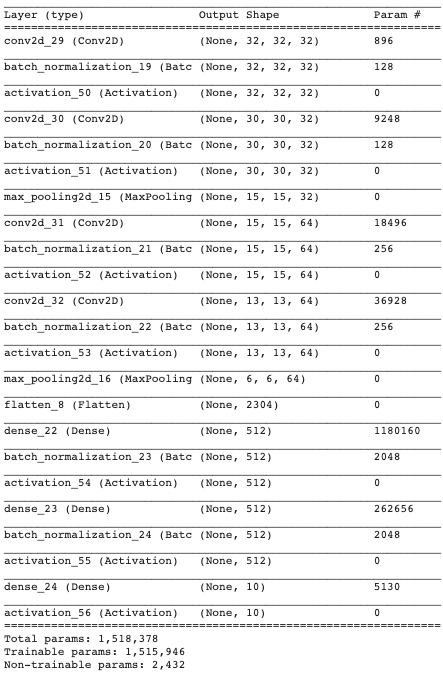
\includegraphics[width=0.28\textwidth]{4.png}
            \caption{Summary of architecture with batch normalization}
    \end{figure}

    Adding batch normalization greatly improved performance as the network as the
    training loss had a final value of 0.1017 with a accuracy of 96.67\%. The validation loss
    ended at 1.3341 with a final accuracy of 78.26\%. The test set reported an accuracy of 77\%.
    The loss and accuracy graphs can be seen below:

    \begin{figure}[H]
        \centering
        \captionsetup{justification=centering}
        \centering
            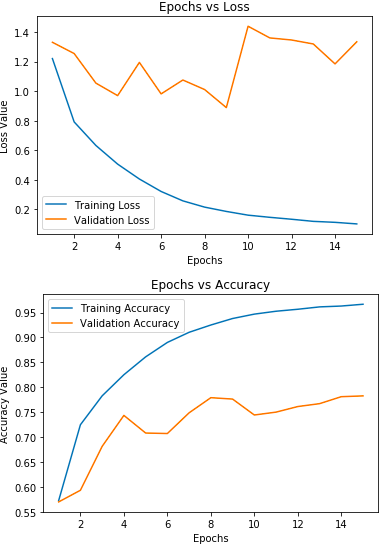
\includegraphics[width=0.28\textwidth]{5.png}
            \caption{Loss and Accuracy curves for batch normalized network}
    \end{figure}

    Although the network is learning much faster it has overfit the data because it performs great
    on the training dataset but fails at the validation and test set.

    \section{Mean Subtraction and Normalization}

    Some code was written to take the mean of each channel (RGB) of each of the total images.
    The mean for each channel was then subtracted from the image. After this we computer the standard
    deviation for each channel (RGB) of each image and normalized the image by it. For example in the first
    image the first pixel of the red channel was 59 and after mean subtraction it became -82.20508 and after
    standard deviation normalization it became -2.0215852. The result on one image is shown below:

    \begin{figure}[H]
        \centering
        \captionsetup{justification=centering}
        \centering
            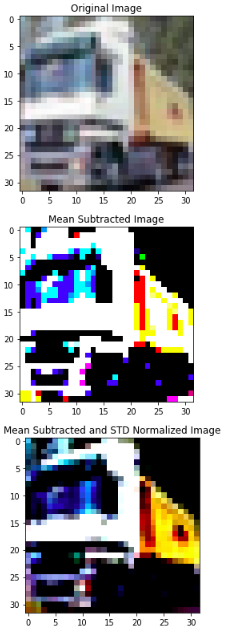
\includegraphics[width=0.16\textwidth]{6.png}
            \caption{Result of mean subtraction and STD normalization}
    \end{figure}

    After doing this the network was retrained and this time the
    training loss had a final value of 0.0606 with a accuracy of 98.13\%. The validation loss
    ended at 1.2952 with a final accuracy of 79.08\%. The test set reported an accuracy of 77.34\%.
    It slightly improved network performance. The image below shows the accuracy and loss curves:

    \begin{figure}[H]
        \centering
        \captionsetup{justification=centering}
        \centering
            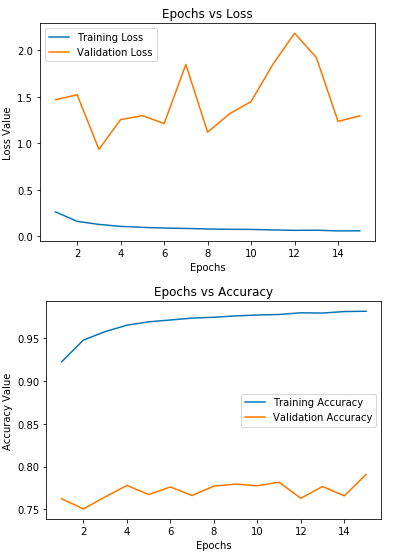
\includegraphics[width=0.28\textwidth]{7.png}
            \caption{Loss and Accuracy curves after doing Mean subtraction and normalization}
    \end{figure}

    \section{Initialization Methods}

    \subsection{Random Uniform and Zero Bias}

    Here I added random uniform initialization to all weights of the network and the biases as zero. With this initializer
    the network started off worse than before and in the same number of epochs it did not do as well as the network without
    initializer. The training loss had a final value of 0.1020 with a accuracy of 96.64\%. The validation loss
    ended at 1.2535 with a final accuracy of 76.86\%. The test set reported an accuracy of 77.00\%. The loss and accuracy
    graphs are shown below.
    
    \begin{figure}[H]
        \centering
        \captionsetup{justification=centering}
        \centering
            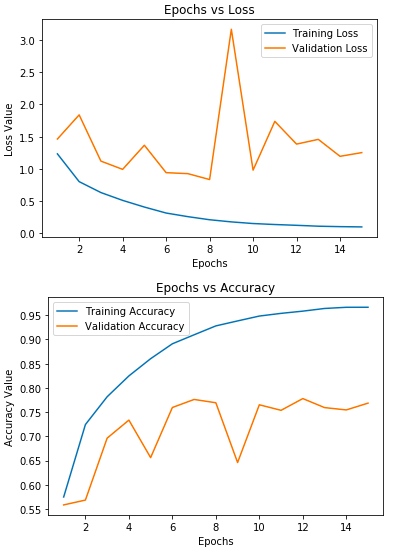
\includegraphics[width=0.21\textwidth]{8.png}
            \caption{Loss and Accuracy curves with random uniform initialization with zero bias}
    \end{figure}

    \subsection{Glorot Normal and Zero Bias}

    Here I added Glorot to all weights of the network and the biases as zero. With this initializer
    the network started off worse than without initializers and in the same number of epochs it did not do as well as the network without
    initializer. However it ended up performing better than the 'Random Uniform' initializer on the training data but worse on test and validation.
    The training loss had a final value of 0.0971 with a accuracy of 96.96\%. The validation loss
    ended at 1.1313 with a final accuracy of 76.76\%. The test set reported an accuracy of 76.23\%. The loss and accuracy
    graphs are shown below. 

    \begin{figure}[H]
        \centering
        \captionsetup{justification=centering}
        \centering
            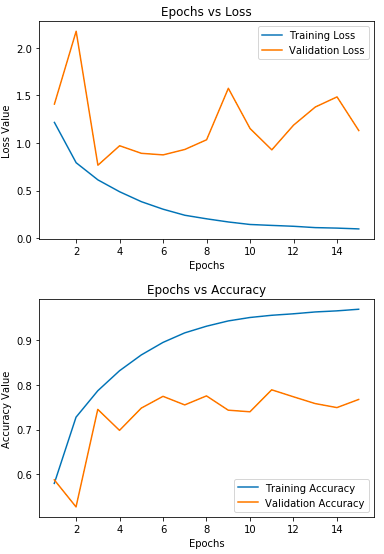
\includegraphics[width=0.21\textwidth]{9.png}
            \caption{Loss and Accuracy curves with Glorot Normal initialization with zero bias}
    \end{figure}

    \subsection{Ones and Zero Bias}

    Here I added ones initialization to all weights of the network and the biases as zero. With this initializer
    the network started off worse than before and in the same number of epochs it did not do as well as the network without
    initializer. It was also the worst initializer. The training loss had a final value of 2.0804 with a accuracy of 19.71\%. The validation loss
    ended at 2.0614 with a final accuracy of 20.38\%. The test set reported an accuracy of 20.88\%. The loss and accuracy
    graphs are shown below.

    \begin{figure}[H]
        \centering
        \captionsetup{justification=centering}
        \centering
            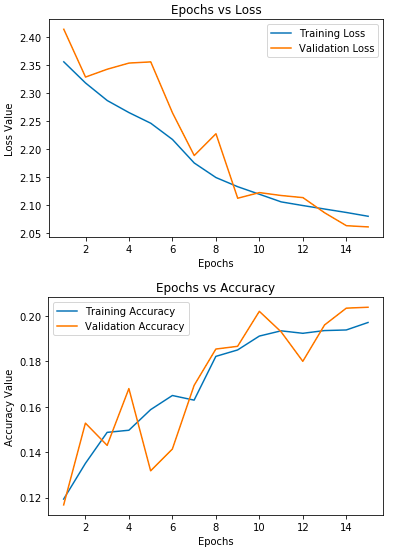
\includegraphics[width=0.21\textwidth]{10.png}
            \caption{Loss and Accuracy curves with Ones initialization with zero bias}
    \end{figure}

    \subsection{LeCun Normal and Zero Bias}

    Here I added the LeCun Normal initialization to all weights of the network and the biases as zero. With this initializer
    the network started off as the best one and in the same number of epochs it did better than the other initializers but not as good as network without an 
    initializer. It was also the worst initializer. The training loss had a final value of 0.1008 with a accuracy of 96.78\%. The validation loss
    ended at 1.1751 with a final accuracy of 76.88\%. The test set reported an accuracy of 76.48\%. The loss and accuracy
    graphs are shown below.

    \begin{figure}[H]
        \centering
        \captionsetup{justification=centering}
        \centering
            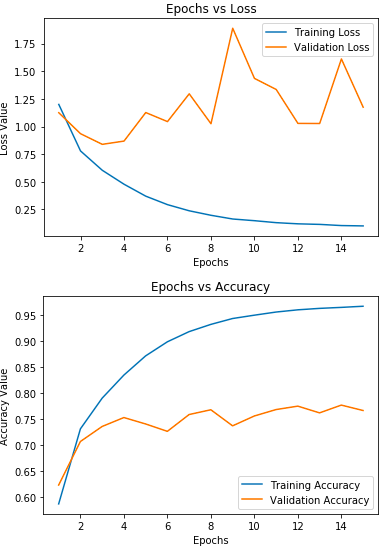
\includegraphics[width=0.21\textwidth]{11.png}
            \caption{Loss and Accuracy curves with Ones initialization with zero bias}
    \end{figure}

    \section{Dropout}

    Here we added 3 dropout layers to the network after we removed the initializer code. The summary is shown below:

    \begin{figure}[H]
        \centering
        \captionsetup{justification=centering}
        \centering
            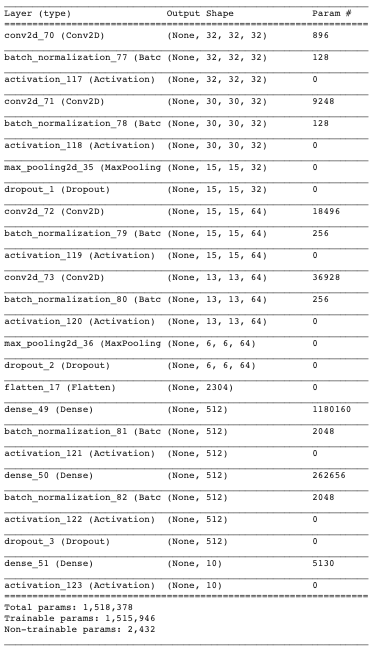
\includegraphics[width=0.35\textwidth]{12.png}
            \caption{Network with Dropout}
    \end{figure}

    Adding dropout greatly improved the network and helped stop the issue of overfitting. In the end the network had a training loss of
    0.7583 and a training accuracy of 75.31\%. The validation loss was 0.6121 and validation accuracy was 79.28\%. The final test set had
    an accuracy of 79.17\%. The loss and accuracy curves are shown below:

    \begin{figure}[H]
        \centering
        \captionsetup{justification=centering}
        \centering
            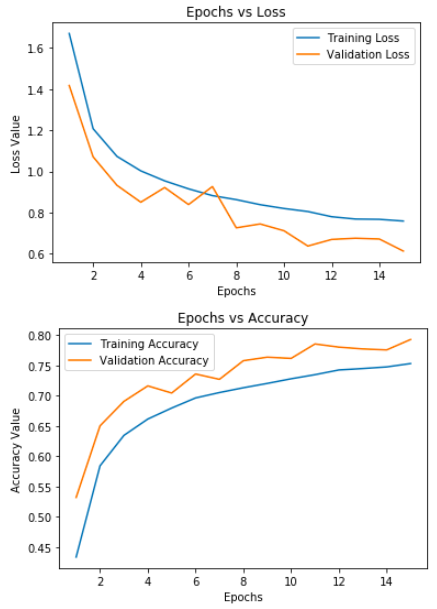
\includegraphics[width=0.2\textwidth]{13.png}
            \caption{Network with Dropout}
    \end{figure}

    \section{Learning Rate and Optimizer}

    So far we have been using the 'RMSprop' optimizer but now we adjust there parameters.

    \subsection{RMSprop with higher learning rate}

    Here the learning rate was increased to 0.002.  In the end the network had a training loss of
    0.8161 and a training accuracy of 74.41\%. The validation loss was 0.6391 and validation accuracy was 79.38\%. The final test set had
    an accuracy of 78.78\%. The network did not perform better with a faster learning rate. Loss and accuracy curve is shown below:

    \begin{figure}[H]
        \centering
        \captionsetup{justification=centering}
        \centering
            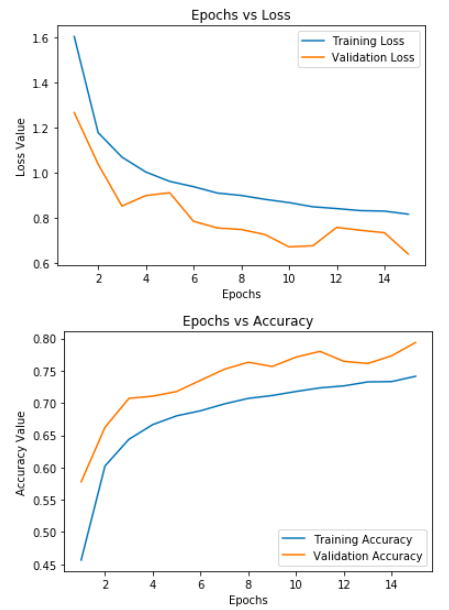
\includegraphics[width=0.2\textwidth]{14.png}
            \caption{Loss and Accuracy curves with increased learning rate of RMSprop}
    \end{figure}

    \subsection{SGD with default parameters}

    Here the optimizer was just switched to SGD. In the end the network had a training loss of
    0.9607 and a training accuracy of 66.17\%. The validation loss was 0.8582 and validation accuracy was 69.96\%. The final test set had
    an accuracy of 69\%. The network did worse that RMSprop. Loss and accuracy curve is shown below:

    \begin{figure}[H]
        \centering
        \captionsetup{justification=centering}
        \centering
            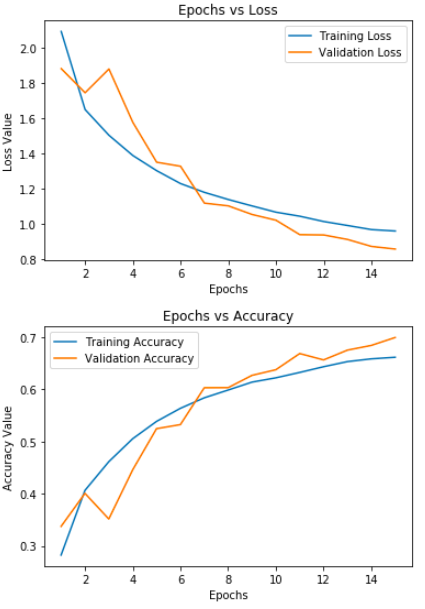
\includegraphics[width=0.2\textwidth]{15.png}
            \caption{Loss and Accuracy curves with SGD}
    \end{figure}

    \subsection{Adam}

    Here the optimizer was just switched to Adam. In the end the network had a training loss of
    0.5902 and a training accuracy of 79.12\%. The validation loss was 0.5763 and validation accuracy was 80.70\%. The final test set had
    an accuracy of 79.93\%. The network with Adam is the best performing so far. Loss and accuracy curve is shown below:

    \begin{figure}[H]
        \centering
        \captionsetup{justification=centering}
        \centering
            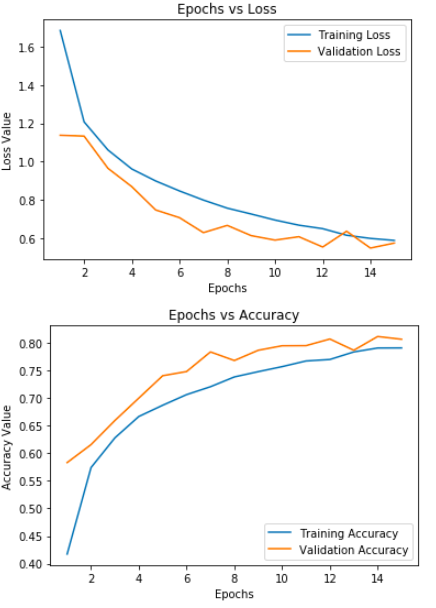
\includegraphics[width=0.2\textwidth]{16.png}
            \caption{Loss and Accuracy curves with Adam}
    \end{figure}

    \subsection{Nadam}

    Here the optimizer was just switched to Nestrov Adam. In the end the network had a training loss of
    0.5835 and a training accuracy of 79.33\%. The validation loss was 0.5379 and validation accuracy was 81.80\%. The final test set had
    an accuracy of 80.38\%. The network with Nadam is the best performing so far. Loss and accuracy curve is shown below:

    \begin{figure}[H]
        \centering
        \captionsetup{justification=centering}
        \centering
            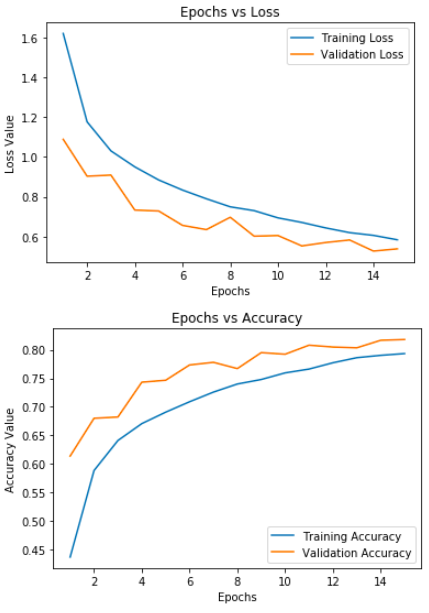
\includegraphics[width=0.2\textwidth]{17.png}
            \caption{Loss and Accuracy curves with Nadam}
    \end{figure}

    \subsection{Nadam with changed parameters}

    Here the Nestrov Adam learning rate was set to 0.008 and the decay is set to 0.01. In the end the network had a training loss of
    0.6739 and a training accuracy of 76.78\%. The validation loss was 0.6381 and validation accuracy was 78.12\%. The final test set had
    an accuracy of 77.75\%. The network with changed parameters did not perform better than the default one. Loss and accuracy curve is shown below:

    \begin{figure}[H]
        \centering
        \captionsetup{justification=centering}
        \centering
            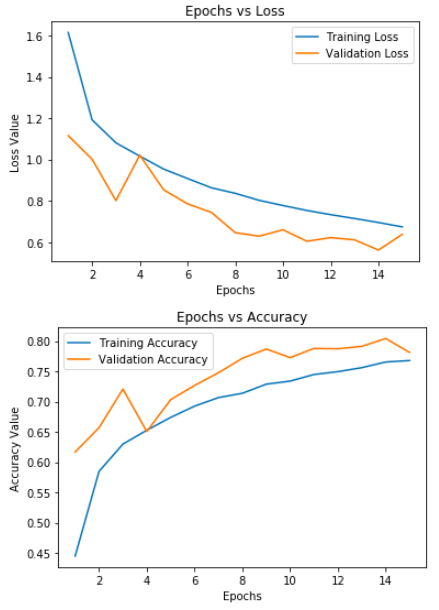
\includegraphics[width=0.2\textwidth]{18.png}
            \caption{Loss and Accuracy curves with Nadam with changed parameters}
    \end{figure}

    \section{Batch Sizes}

    So far the batch size being used has been 32.

    \subsection{Batch size of 128}

    I used the network with Nadam and changed the batch size to 128. In the end the network had a training loss of
    0.5078 and a training accuracy of 82.20\%. The validation loss was 0.5273 and validation accuracy was 82.06\%. The final test set had
    an accuracy of 81.39\%. This network is the best performing so far. Loss and accuracy curve is shown below:

    \begin{figure}[H]
        \centering
        \captionsetup{justification=centering}
        \centering
            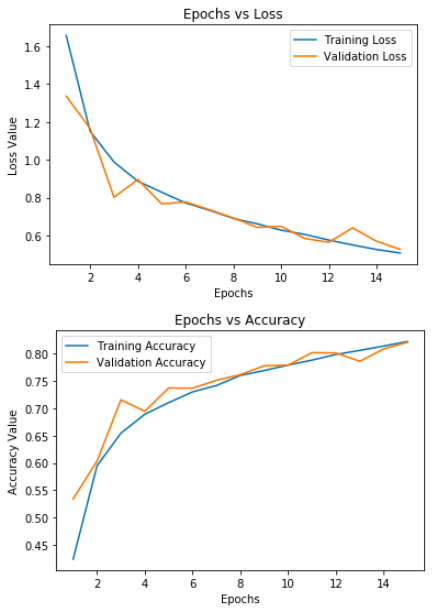
\includegraphics[width=0.2\textwidth]{19.png}
            \caption{Loss and Accuracy curves with batch size of 128}
    \end{figure}

    \subsection{Batch size of 512}

    Now the batch size is changed to 512. In the end the network had a training loss of
    0.5369 and a training accuracy of 81.15\%. The validation loss was 0.6154 and validation accuracy was 79.64\%. The final test set had
    an accuracy of 78.93\%. This network did not perform better. Loss and accuracy curve is shown below:

    \begin{figure}[H]
        \centering
        \captionsetup{justification=centering}
        \centering
            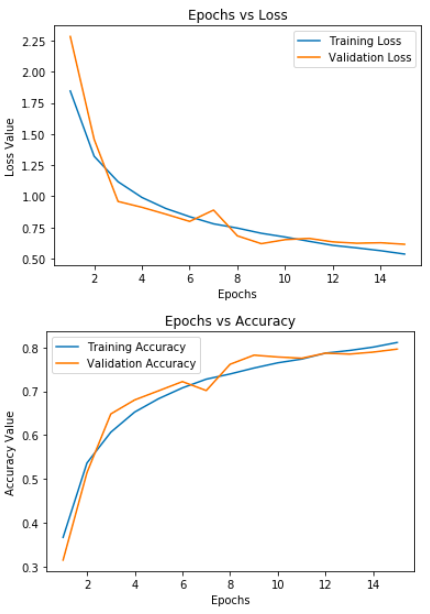
\includegraphics[width=0.2\textwidth]{20.png}
            \caption{Loss and Accuracy curves with batch size of 512}
    \end{figure}

    \section{Results}

    In the end the best network used the 'Nestrov Adam' optimizer and had a batch size of 128. Its summary is shown in figure 12 and results details are in VIII.A . Throughout the
    homework only 20 epochs were used. The final test accuracy was 81.39\%
\end{document}